\documentclass[11pt]{article}
\usepackage{geometry}                % See geometry.pdf to learn the layout options. There are lots.
\geometry{letterpaper}                   % ... or a4paper or a5paper or ... 
%\geometry{landscape}                % Activate for for rotated page geometry
%\usepackage[parfill]{parskip}    % Activate to begin paragraphs with an empty line rather than an indent
\usepackage{graphicx}
\usepackage{amssymb}
\usepackage{epstopdf}
\usepackage{amsmath}
\usepackage{nameref}
\usepackage{subcaption}
\usepackage[section]{placeins}
\usepackage[innerleftmargin = 4pt, innerrightmargin = 4pt, innertopmargin = 4pt, innerbottommargin = 4pt]{mdframed} 

\newcommand*{\fullref}[1]{\hyperref[{#1}]{ \textbf{\ref*{#1}.~\nameref*{#1}}}}
\newcommand{\todo}[1]{{\color{green}{#1}}}
\newcommand{\whw}[1]{{\color{blue}{#1}}}

\graphicspath{{./graphics/}}

\DeclareGraphicsRule{.tif}{png}{.png}{`convert #1 `dirname #1`/`basename #1 .tif`.png}

\usepackage[style=numeric-comp, backend=bibtex, sorting=none, maxbibnames=20,isbn=true]{biblatex}
\usepackage[colorlinks=true,linkcolor=black,urlcolor=gray,citecolor=black]{hyperref}
\addbibresource{./supporting_files/biblio.bib}

\title{Multilayer Modularity Belief Propagation} %need a better title 
\author{William Weir and Benjamin Walker} 
\date{\today}                                           % Activate to display a 
\begin{document}
\maketitle

\section{Abstract} 

\section{Introduction}

%\begin{enumerate}
%\item Background on Belief Propagation
%\item Description of modularity
%\end{enumerate}

One popular heuristic for community detection involves optimizing a quantity developed by Newman and Girvan known as modularity \cite{Newman:2003ep}.  Modularity compares the observed edges internal to the groups of a partition to the number expected under a random configuration model of the network.  The formula for modularity modularity on a weighted network given by adjacency matrix $A_{i,j}$ is given by \cite{Newman:2003ep}
\begin{equation}
\label{eq:mod}
Q(\gamma)=\frac{1}{2m}\sum_{i,j}{\left( A_{ij}-\gamma \frac{k_ik_j}{2m}\right)\delta(c_i,c_j)}\,,
\end{equation}

Where $k_i=\sum_j{A_{i,j}}$ is the weighted degree (strength) of node i, $m=\frac{1}{2}\sum{A_{i,j}}$ is the total edge weight of the network, and $\gamma$ is the resolution parameter introduced by Reichardt and Bornholdt \cite{Reichardt:2006eh} that sets the scale of the communities identified. Setting $\gamma=1$ gives the original modularity formulation in \cite{Newman:2003ep}.  In general, maximizing the function over the combinatorially large space of possible partitions is \emph{NP-Hard} and most methods attempt to find a locally optimal solution. 

\subsection{ Modularity Belief Propagation}
One of the crucial problems with the optimization of modularity as a means of community detection is that partitions of high modularity often exist even in completely random networks.  Recently, Zhang and Moore applied the tools of statistical physics to overcome several of the challenges associated with previous heuristics aiming to maximize modularity\cite{Zhang:2014gea}.  They approach the problem as a spin-glass system with the energy given by $ \mathcal{E}=-mQ(\{t\}) $ and a Gibbs distribution by : 

\begin{equation}
P(\{t\})  \propto e^{\-\beta {\mathcal{E}} (\{t\} )}
\label{eq:gibbsprob}
\end{equation}

where $\{t\} = [t_1,\hdots,t_N]; t_i \in \{1, ..., q\}$ being an assignment of the nodes in a network into $q$ communities, and $\beta$ representing an inverse temperature parameter determining how the probability is spread throughout the different states.  As $\beta \rightarrow \infty $, the low temperature regime, only the partitions with the globally maximum modularity have non-zero probabilities.  They suggest that instead of attempting to maximize modularity directly, community assignments should be made on the basis of the marginals of such a distribution in Eq.~ \ref{eq:gibbsprob}.  There are several tools to compute the marginals of such the distribution such as Markov Chain Monte Carlo sampling, Gibb's sampling, and the class of algorithms called \textit { Belief Propagation} ( also known as the cavity method), for which the derive the following update conditions: 

\begin{equation}
\psi^{i \to k }_t \propto \exp {\left [ \frac{\beta d_i }{2m}\theta_t  + \sum_{j\in \partial i \\ k} \log{1+\psi^{j \to i }_t(\exp^{\beta}-1)} \right ]}
\label{eq:modbp}
\end{equation}

Where $\theta_t=\sum_j{d_j\psi^{j}} $  and $\partial i$ denotes the neighbors of node $i$ in the graph.  We refer to Zhang and Moore's algorithm as \textit{modbp}. 

Zhang and Moore posit that in the event that if there exists several global maximum that are widely separated in the space of partitions ( \textit{i.e.} uncorrelated), belief propagation will oscillate between these partitions and fail to converge.  The demonstrate this by showing the absence of a non-trivial retrieval phase for random ER graphs without structure.  

\subsection{Selection of Number of Communities \label{numcom}}

One issue with many community detection algorithms is in the selection of the appropriate number of communities.  In the context of modularity, adjusting $\gamma$ , ``resolution parameter", in Eq.~\ref{eq:mod} can reveal communities of different scale and size therefore overcoming the ``resolution limit of detection" first raised by \cite{Fortunato:2007js}.  Zhang and Moore do not include a resolution parameter in deriving their \textit{modbp} algorithm (thereby implicitly setting $\gamma=1$), and suggest an alternative approach to selecting the appropriate number of communities.  They show in several examples that the maximum modularity achieved in the retrieval phase of the algorithm peaks at the appropriate number of communities, with no increase in $\hat{Q}$, the retrieval modularity once the appropriate number of communities is selected.  However, this requires running \textit{modbp} for many possible value of $q$, number of community assignments.  

There have been two other approaches to selecting the appropriate number of communities using \textit{modbp} without having to run the algorithm at many values of q.  Both approaches involve selecting a $q_{\text{max}}$, the largest possible number of communities, and then using the marginal probabilities of assignments to evaluate the true number of communities.  Lai \textit{et al.} noted that in the event that q is too large, many of the marginal community assignments will be highly correlated, and highly correlated states (community assignments) can be condensed into a single group \cite{Lai:2016el}.  Similarly in Ref~\cite{Schulke:2015hq}, they condense the community assignments on the basis of the average distance between the marginals across all nodes in the network.  In practice, we have that choosing the number of communities the number of communities this way all but obliterates the retrieval phase if $q_{\text max}$ is chosen too high above the actually number.  We have implemented the method in Ref~\cite{Schulke:2015hq}, letting the number of communities float up to a pre-specified $q_{\text{max}}$ (see Methods), and show that incorporation of a resolution parameter, $\gamma$ restores the width of the retrieval phase and returns closer to the correct number of communities.  

\subsection{Multilayer Modularity Belief Propagation}
An extension of modularity for the multilayer case was developed by Mucha~\textit{et al.} to incorporated the coupling between the layers \cite{Mucha:2010vk}.  Using an analysis of modularity from a Laplacian dynamics perspective, they developed a null model for multilayer networks and gave the following formula for multilayer modularity: 

\begin{equation}
Q(\gamma,\omega)=\sum_{i,j} \left( A_{ij} - \gamma P_{ij} + \omega C_{ij} \right)\delta(c_{i},c_{j})
\label{eq:multimod}
\end{equation}

While there are belief propagation models for the multilayer context, \cite{Ghasemian:2016hg} for example, to date there has not been an extension of \textit{modbp} to the multilayer context.  

In this paper, we have extended Zhang and Moore's \textit{modbp} method in three important ways.  We allow for the presence of weighted edges, which can greatly influence the communities detected ( see \whw{references needed} ).  We have incorporated a resolution parameter, $\gamma$ into the algorithm and show that this can create a wider retrieval phase and achieve better performance in the case where the number of communities is not known \textit{ a priori}.  Finally, we have extended \textit{modbp} to the multilayer framework developed by Mucha~\textit{et al.} \cite{Mucha:2010vk} and demonstrated the use of this tool on both synthetic and real world data.  We refer to our tool as \textit{multimodbp} which can be used on both Multilayer networks and single-layer networks.  We have developed a python package, implementing our method in a fast, efficient manner and interfaces with other standard networks tools. 




\section{Results}

\subsection{Single Layer}

We begin by examining how our modifications effect the ability of \textit{modbp} to detect communities within synthetically generated data in the single layer case.  For single layer networks, our method collapses down to Zhang and Moore's with two main differences (see also \fullref{methods}):   
\begin{enumerate}
\item We have included a resolution parameter, $\gamma$ that adjusted the relative balance of the terms in the update equation.  Like other implementations of modularity this effectively controls the size of the partitions identified within the retrieval phase.
\item We have set an upper limit on the number of communities, $q_{\text max }$ and have incorporated the approach Ref~\cite{Schulke:2015hq} to select an effective number of communities based on the overlap of the marginal (see \fullref{numcom})
\end{enumerate}

\subsubsection{Single Layer Stochastic Block Model}
%\begin{figure}[htbp]
%\begin{center}
%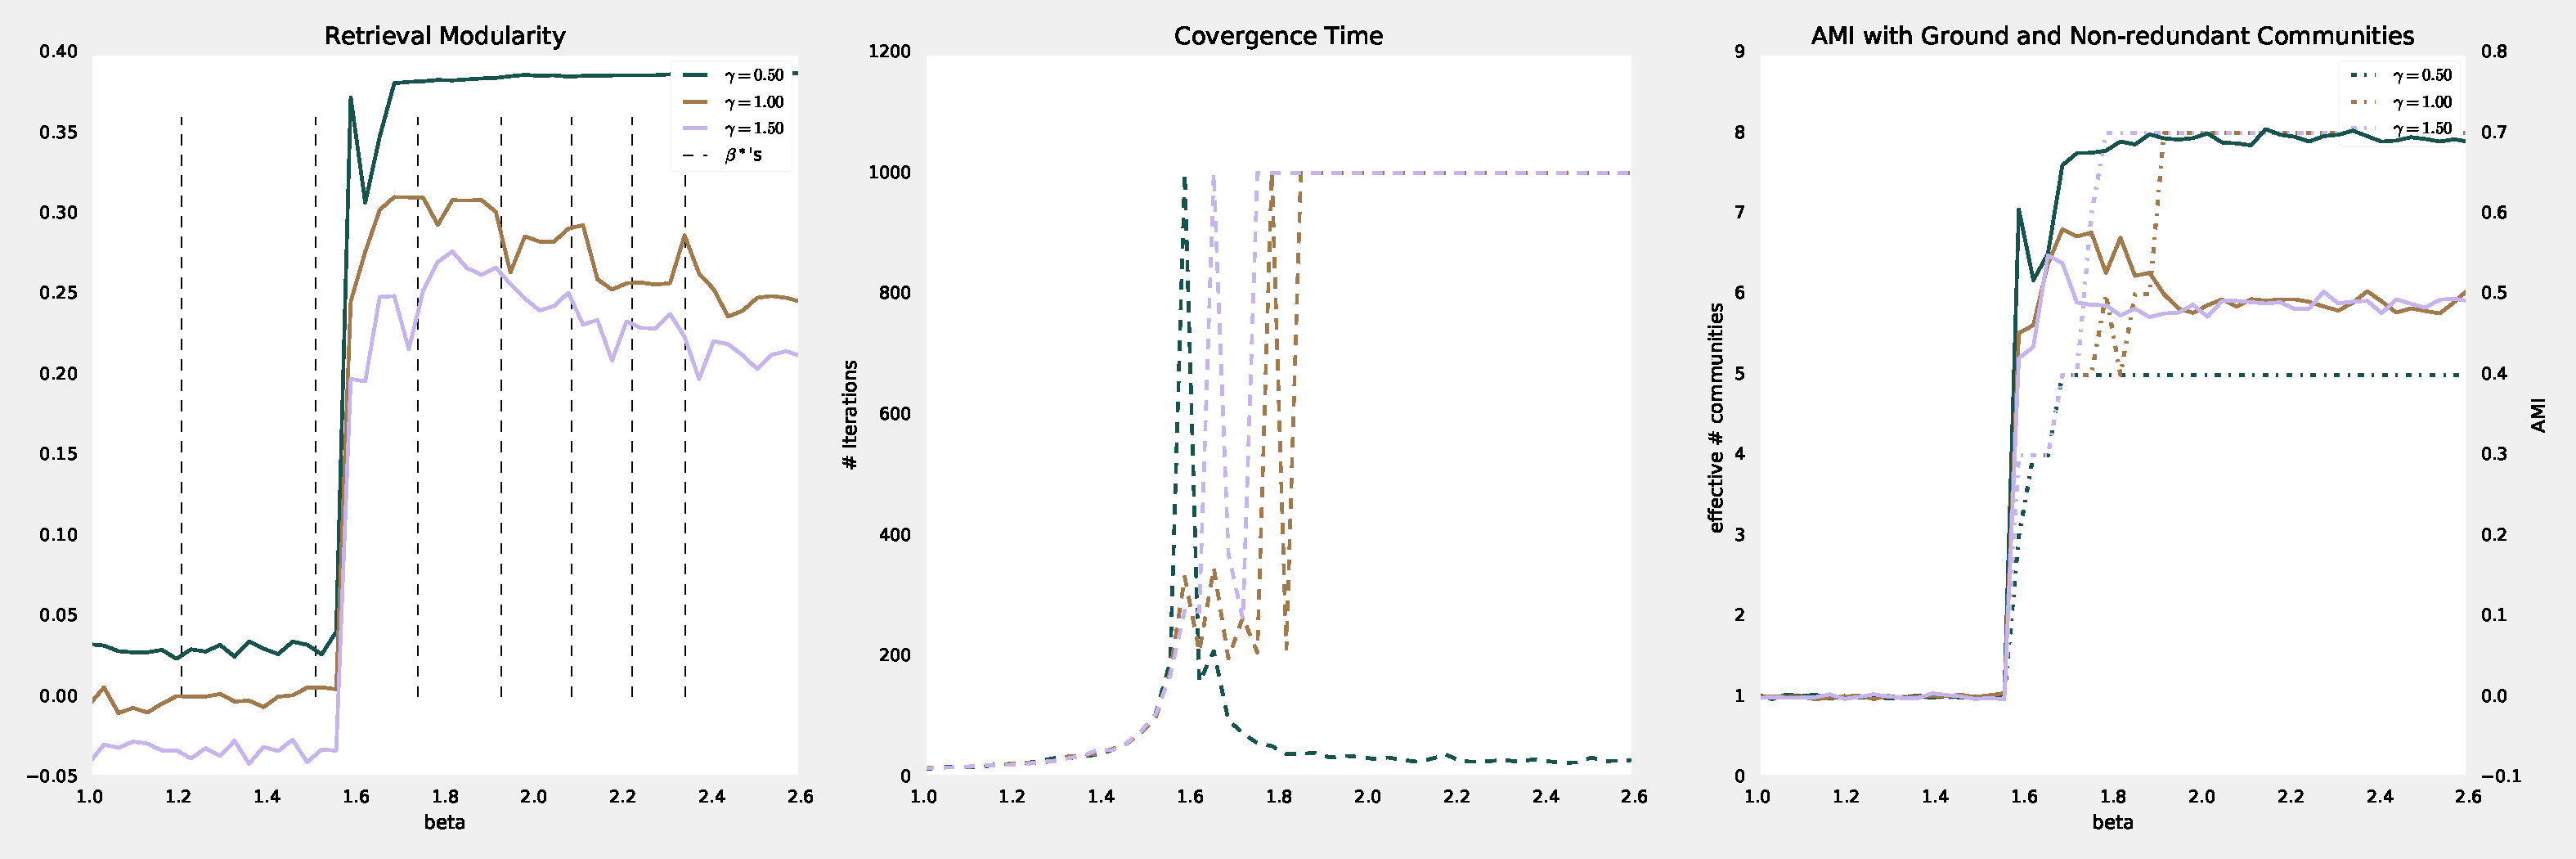
\includegraphics[width=\linewidth]{fourcom_varyinggamma4c.pdf}
%\caption{ \textbf{A} ) retrieval modularity, $\hat{Q}$ for partitions identified at convergence of \textbf{multimodbp}  \label{fig:4comeven}
%}
%\end{center}
%\end{figure}
% This is wil one large figure for this section 
\begin{figure}[!htb]
\centering
\begin{subfigure}{\textwidth}
	\begin{mdframed}
		\includegraphics[width = .74\textwidth]{fourcom_even_varyinggamma4c.pdf}
		\includegraphics[width = .24\textwidth]{igraph_even_commlayout4c.pdf}
		\hspace{-.2in}
		\begin{minipage}[c]{0.001\textwidth}
		\caption{ \label{fig:igeven}}
		\end{minipage}%
	\end{mdframed}
\end{subfigure}%

\begin{subfigure}{\textwidth}
	\begin{mdframed}
		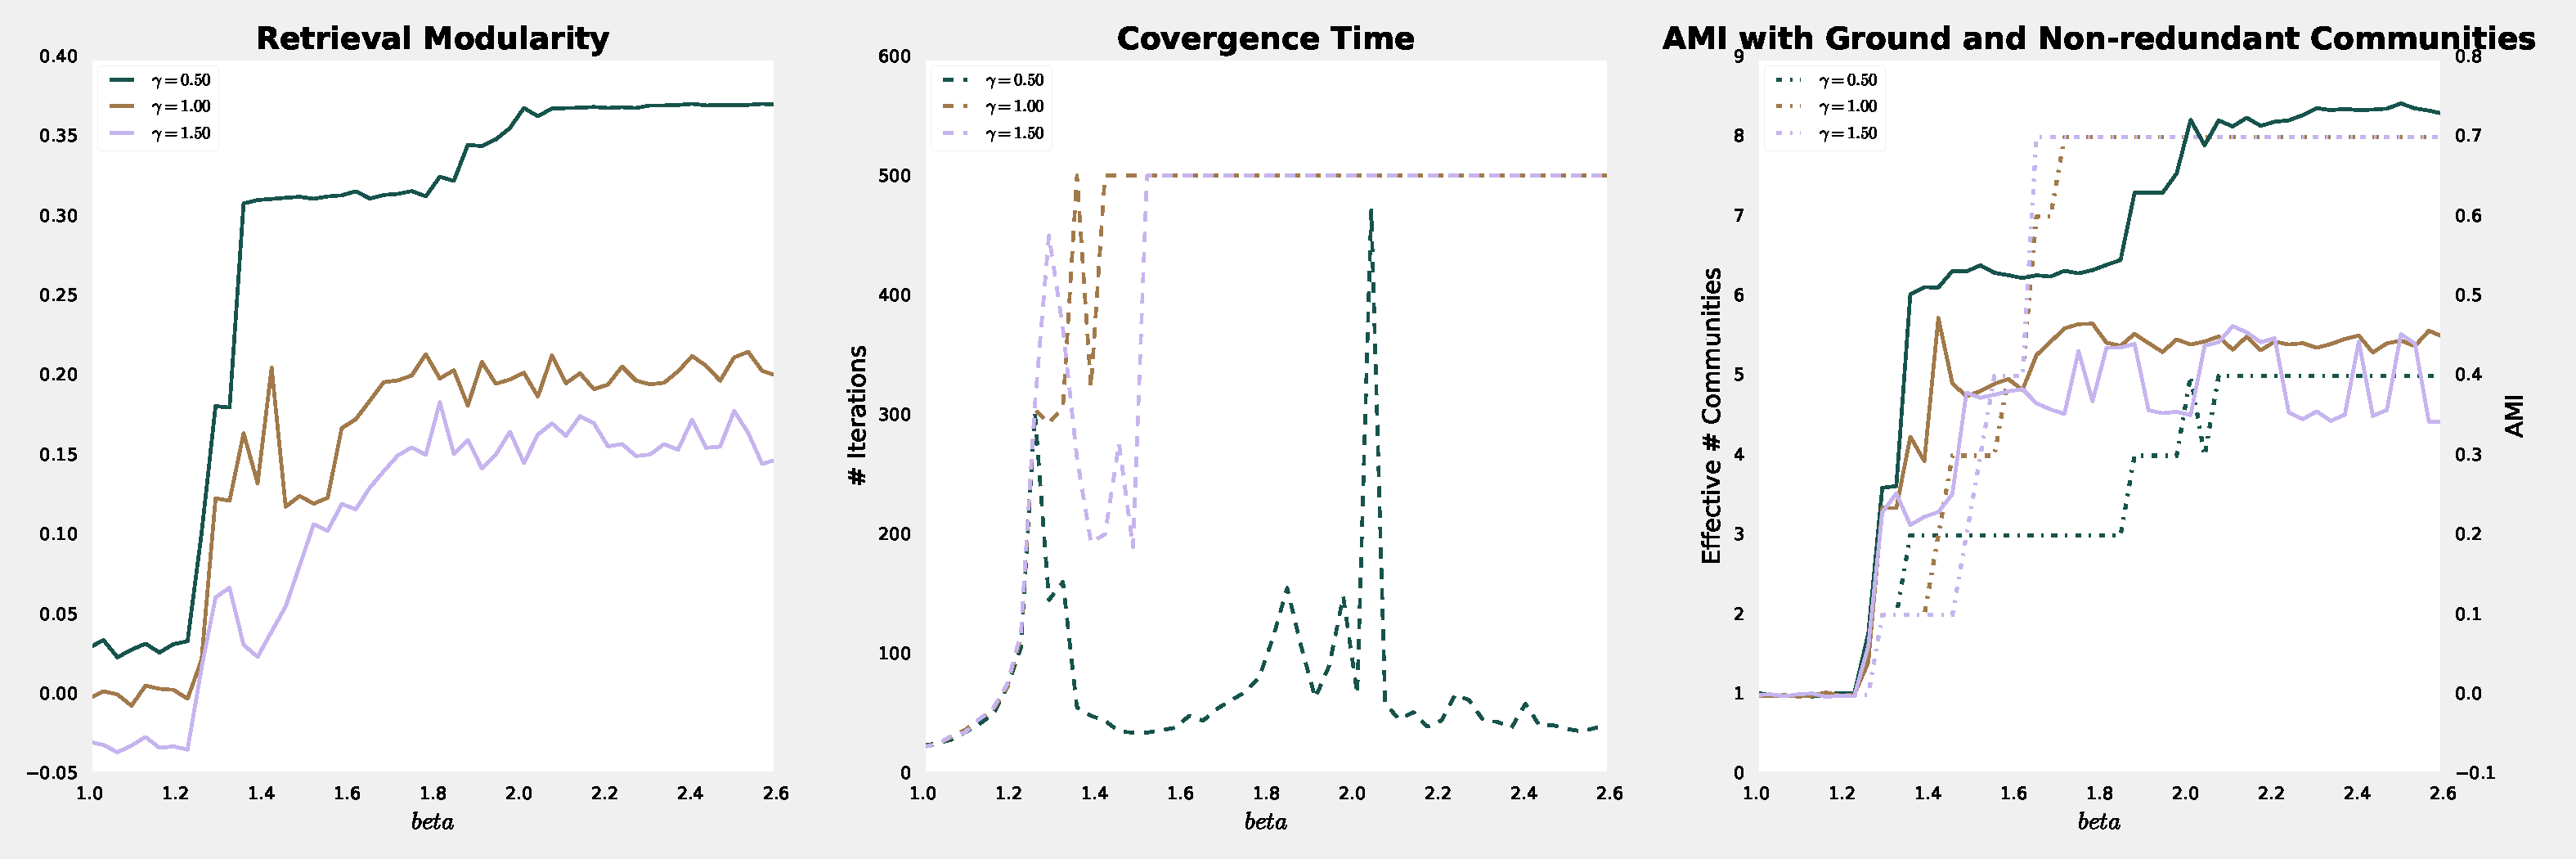
\includegraphics[width = .74\textwidth]{fourcom_uneven_varyinggamma4c.pdf}
		\includegraphics[width = .24\textwidth]{igraph_uneven_commlayout4c.pdf}
		\hspace{-.2in}
		\begin{minipage}[c]{0.001\textwidth}
		\caption{\label{fig:iguneven}}
		\end{minipage}\hfill%
		\end{mdframed}
\end{subfigure}
\vspace{-.1in}
\caption { Demonstration of \textit{multimodbp} on two realization of SBM model.  From left to right the plots show the retrieval modularity, number of iterations to convergence, and the AMI of the retrieved partition with known community assignments and the effective number of communities.  The black dotted lines denote the values of $\beta^*$ for values of $q$ ranging from 2 to $q_{\text{max}}$ (see \ref{eq:bstar}).  \textbf{(a)} 4 community SBM with $n=1000$,  $\epsilon=\frac{p_{out}}{p_{in}}=.1$, $c_{avg}=4$, and even community sizes and  \textbf{(b)} and 4 community SBM with $n=1000$,  $\epsilon=.1$, $c_{avg}=4$, with  uneven community sizes ( $\nu = [ 350,150,350,150]$ ) \label{fig:singlelayer} } 
\vspace{-.2in}
\end{figure}
We examine the behavior of \textit{multimodbp} on realization of a four community stochastic block model for different values of $\gamma$.  First, we show that in the setting with several smaller communities, a higher value of $\gamma$ produces a much wider retrieval phase and thus makes detection of communities more robust to selection of $\beta$.  We generated a single realization of an SBM and scanned a range of $\beta$ values to characterize the behavior of the algorithm seen in \textbf{Figure~\ref{fig:singlelayer}}.  The retrieval modularity seen in \textbf{Figure~\ref{fig:igeven}} shows a clear plateau for $\gamma=.5$ (right most panel), corresponding with a broad retrieval phase (middle panel) that is absent at $\gamma=1$.  The AMI (left most panel) is clearly higher for all values of $\gamma$ within the retrieval phase.  What's more, the number of communities identified for $\gamma=.5$ plateaus at 5, which is more closely aligned with the underlying model (really there are only 4 main communities show in far right panel of \textbf{Figure~\ref{fig:igeven}}).  

We also tested the performance of the algorithm in the case where the sizes of the planted communities were uneven, shown in \textbf{Figure~\ref{fig:iguneven}}.  The results here were similar though even more striking.  There is a small retrieval phase for $\gamma=1$, but it is much smaller than that of $\gamma=.5$ and the AMI is again consistently lower.  For $\gamma=.5$ we actually detect two retrieval phases, the first one in which only nodes within the two larger communities are labelled correctly.  Then as $\beta$ increases the smaller two communities also become identifiable.  This is consistent with the multiphase behavior observed in \cite{Schulke:2015hq}, though we note that in this example, the phase transition is only observed in a particular $\gamma$ regime.

\subsubsection{ NCAA Division I-A College Football Network }
 
 We also look at how incorportation of the resolution parameter affects the ability of \textit{multimodbp} to detection community structure on real world network.  As 
 
 
 To look at how the value of $\gamma$ effects the retrieval phase, we ran \textit{multimodbp} for a range of $\gamma$ value and examined the minimal number of iterations in the retrieval phase shown  in \textbf{Figure~\ref{fig:footballgamma}}.  For each value of $\gamma$, \textit{multimodbp} was run over ten values in $\beta \in [1.5,2.5]$, and values calculated at the $\beta$ corresponding to the minimum number of iterations within this range.  Runs that did not converge after 500 iterations suggest that for that value of $\gamma$ the retrieval phase was either very small or nonexistent.  Furthermore, \textbf{Figure~\ref{fig:footballgamma}} demonstrates that the AMI of the retrieved partition increases as a function of $\gamma$  from $\gamma=1$ up until is plateaus form $\gamma=[1.7,3.4]$ at a stable 11 community solution (show in far right panel).    
     
 \begin{figure}[!htbp]
\begin{center}
	\begin{mdframed}
		\includegraphics[width = .66\textwidth]{football_gamma_scan.pdf}
		\includegraphics[width = .33\textwidth]{igraph_american_football.pdf}
%		\hspace{-.2in}
%		\begin{minipage}[c]{0.001\textwidth}
%		\caption{ \label{fig:igeven}}
%		\end{minipage}%
	\end{mdframed}
\caption{ \label{fig:footballgamma}}
\end{center}
\end{figure}   

%	\begin{mdframed}
%		\includegraphics[width = .74\textwidth]{fourcom_even_varyinggamma4c.pdf}
%		\includegraphics[width = .24\textwidth]{igraph_even_commlayout4c.pdf}
%		\hspace{-.2in}
%		\begin{minipage}[c]{0.001\textwidth}
%		\caption{ \label{fig:igeven}}
%		\end{minipage}%
%	\end{mdframed}
%    
%\begin{figure}[htbp]
%\begin{center}
%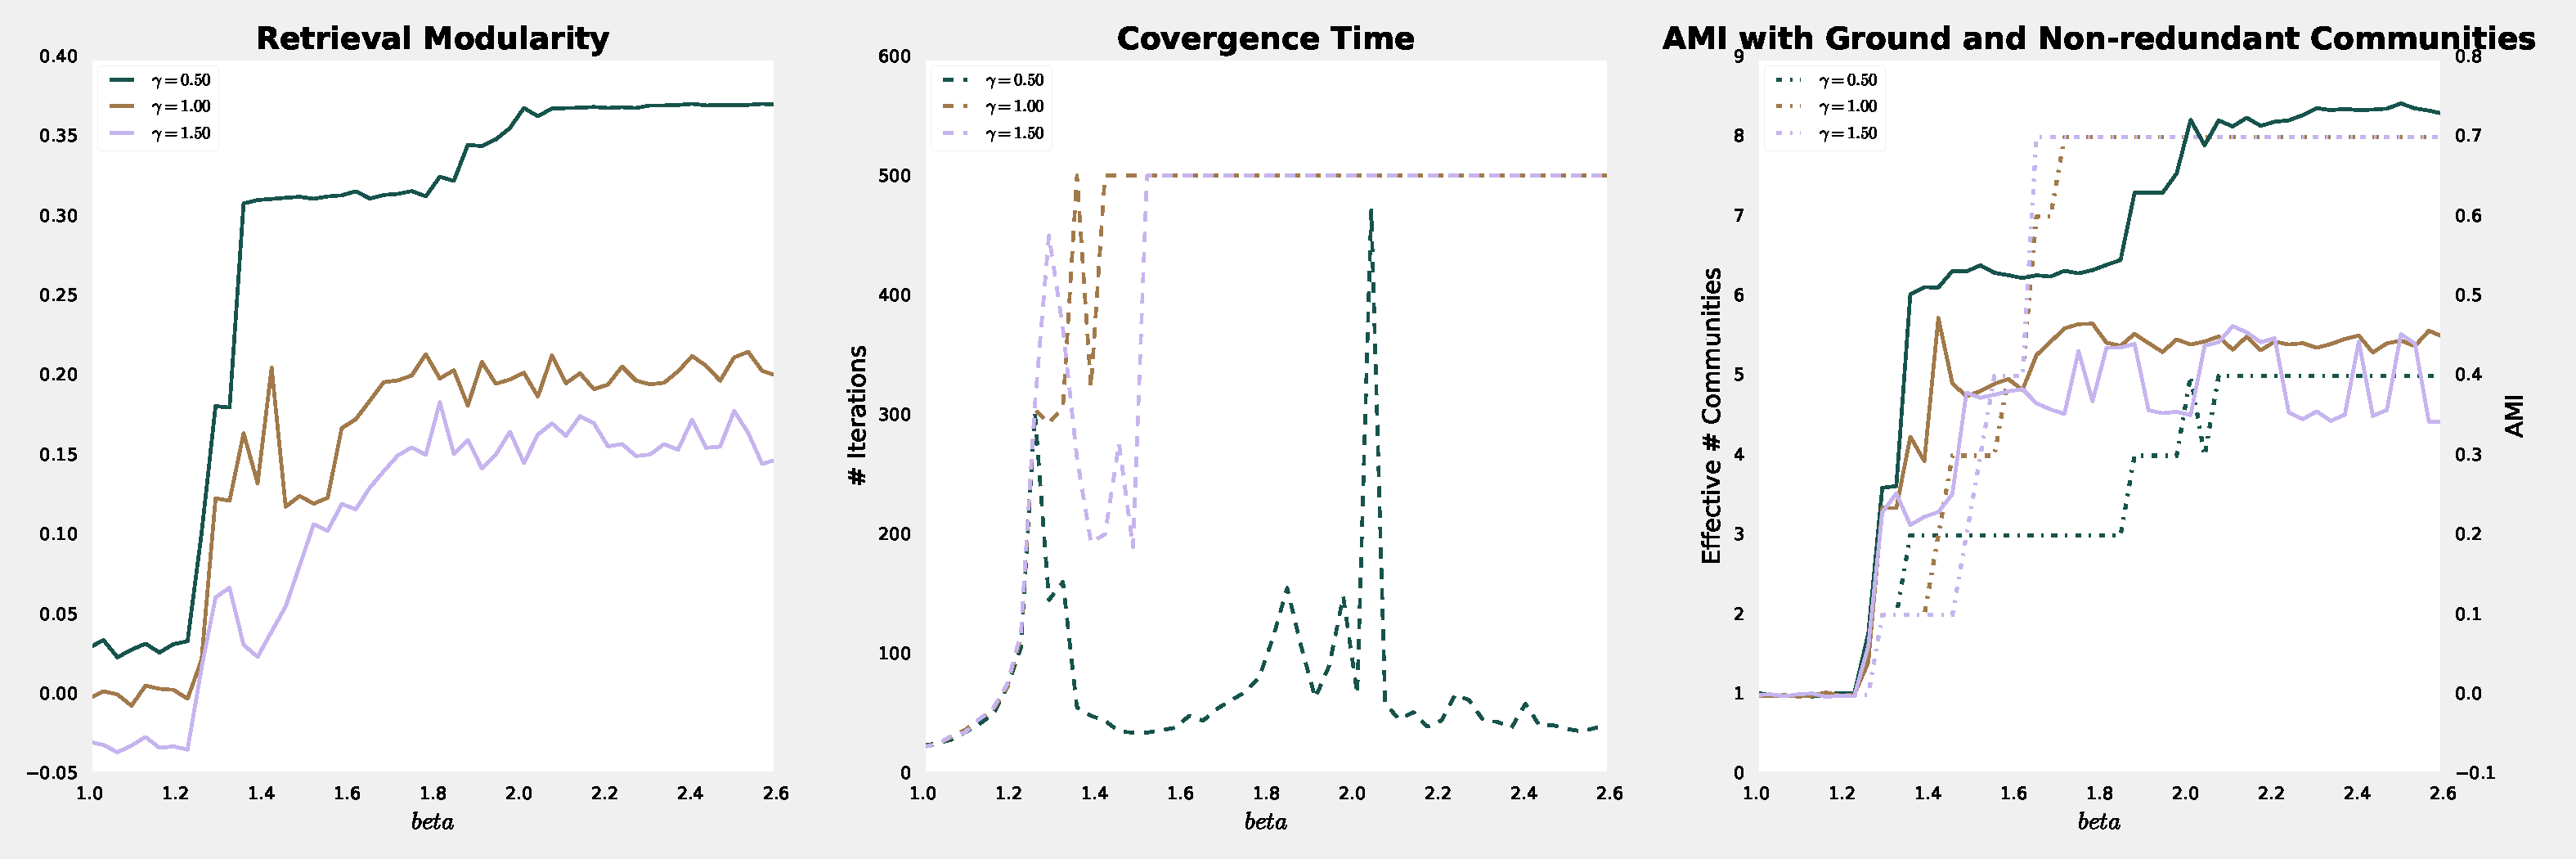
\includegraphics[width=\linewidth]{fourcom_uneven_varyinggamma4c.pdf}
%\caption{caption \label{fig:4comuneven}
%}
%\end{center}
%\end{figure}
%
%\begin{figure}[h]
%\centering
%\begin{subfigure}{.4\textwidth}
%	\begin{mdframed}
%%		\caption{ \label{fig:pfamdoms}}
%		\includegraphics[width = \textwidth]{igraph_even_commlayout4c.pdf}
%%		\hspace{-3.7in}
%		\begin{minipage}[c]{0.01\textwidth}
%		\caption{ \label{fig:igeven}}
%		\end{minipage}\hfill%
%	\end{mdframed}
%\end{subfigure}%
%\begin{subfigure}{.4\textwidth}
%	\begin{mdframed}
%		\includegraphics[width = \textwidth]{igraph_uneven_commlayout4c.pdf}
%%		\hspace{-3.6in}
%		\begin{minipage}[c]{0.01\textwidth}
%		\caption{\label{fig:iguneven}}
%		\end{minipage}\hfill%
%		\end{mdframed}
%\end{subfigure}
%\vspace{-.1in}
%\caption {  \textbf{(a)}  \textbf{(b)}  } 
%\vspace{-.2in}
%\end{figure}

%\begin{figure}[htbp]
%\begin{center}
%\includegraphics[width=.45\linewidth]{igraph_even_commlayout.pdf}
%\includegraphics[width=.45\linewidth]{igraph_uneven_commlayout.pdf}
%\caption{Layout of SBM colored by communities identified within the retrieval phase. \label{fig:4comuneven}}
%\end{center}
%\end{figure}

\FloatBarrier
\subsection{Multilayer}

%as well as the energy function optimized  



\section{Discussion}
\section{Conclusion}

\section{Method Description \label{methods}}

We have made two major modifications to Zhang and Moore's original \text{modbp} update equations.  First, we have included a resolution parameter, $\gamma$ which decouples the contribution of the two terms within the update equation.  Second, we introduce an additional term to account for interlayer edges in a term that is nearly identical to the intralayer terms.  It includes it's own interlayer coupling parameter, $\omega$ that influence's the relative contribution of this term.  
%\begin{equation}
%\psi^{i \to k }_t \propto
% \exp {\left [ \gamma \frac{\beta d_i }{2m}\theta_t  + \sum_{j\in \partial i \\ k} \log{(1+\psi^{j \to i }_t(e^{\beta}-1))} + \sum_{j\in \partial i \\ k} \log{(1+\psi^{j \to i }_t(e^{\omega\beta}-1))}\right ]}
%\label{eq:multimodbp}
%\end{equation}


\begin{equation}
\psi^{i \to k }_t \propto \begin{cases}  \exp {\left [ \gamma \frac{\beta d_i }{2m}\theta_t  + \sum_{j\in \partial i \setminus k} \log{(1+\psi^{j \to i }_t(e^{\beta}-1))} \right]} & (i,k) \in \mathcal{E}_{\text{intra}}\\ 
\exp {\left [  \sum_{j\in \partial i \setminus k} \log{(1+\psi^{j \to i }_t(e^{\omega\beta}-1))}\right ]} & (i,k)\in \mathcal{E}_{\text{inter}} \end{cases}
\end{equation}

%\begin{equation}
%\psi^{i \to k }_t \propto \begin{cases}   \exp {\left [ \gamma \frac{\beta d_i }{2m}\theta_t  + \sum_{j\in \partial i \\ k} \log{(1+\psi^{j \to i }_t(e^{\beta}-1))} \right ]} & x = 0\\ 
%\exp {\left [  \sum_{j\in \partial i \\ k} \log{(1+\psi^{j \to i }_t(e^{\omega\beta}-1))} \right ]} & x > 0 \end{cases}
%\label{eq:multimodbp}
%\end{equation}


Where $\mathcal{E}_{\text{inter}}$, denotes the interlayer edges, while $\mathcal{E}_{\text{intra}}$ is the set of interlayer edges.  While, we have demonstrated \textit{multimodbp} in the context of a specific multilayer topology, that is the multiplex network, our formulation is flexible enough to handle any type of multilayer networks with two classes of edges.  In principle, the method could even be extended to many edge types, each with their own coupling parameter, $\omega_i$.  

\subsection{Identification of $\beta$}



\begin{equation} \label{eq:bstar}
\beta^*=\log\left(\frac{q}{(\sqrt{c}-1)}+1\right)
\end{equation}

Where $c=\frac{<d^2>}{<d>}-1$ is the excess degree.  Based 


\printbibliography

%\subsection{}



\end{document}  
